\documentclass[10pt]{article}
\usepackage{../EllioStyle}
\usepackage{listings}
\usepackage{multicol}

\definecolor{codegreen}{rgb}{0,0.6,0}
\definecolor{codegray}{rgb}{0.5,0.5,0.5}
\definecolor{codepurple}{rgb}{0.58,0,0.82}
\definecolor{backcolour}{rgb}{0.95,0.95,0.92}
\DeclareMathOperator*{\argmin}{arg\,min}

\usepackage[small]{titlesec}

\lstdefinestyle{mystyle}{
%    backgroundcolor=\color{backcolour},   
    commentstyle=\color{codegreen},
    keywordstyle=\color{magenta},
    numberstyle=\tiny\color{codegray},
    stringstyle=\color{codepurple},
    basicstyle=\ttfamily\footnotesize,
    breakatwhitespace=false,         
    breaklines=true,                 
    captionpos=b,                    
    keepspaces=true,                 
    numbers=left,                    
    numbersep=5pt,                  
    showspaces=false,                
    showstringspaces=false,
    showtabs=false,                  
    tabsize=2
}

\titlespacing{\section}{0pt}{0pt}{0pt}
\setlength{\parskip}{8pt}

\title{Notesheet}
\author{Elliott Pryor}
\date{October 7 2021}

\rhead{Notesheet for Exam 1}

\begin{document}
\multicols{2}


\section{Global Alignment}
The goal is to find the optimal alignment of two strings.
This can be edit distance: where $\delta(x, x) = 0$, $\delta(x, y) = -1$
Which essentially counts the number of differences in the string. Or it can be a more complicated metric.
The global alignment score problem has $\delta(x, x) = 2$, $\delta(x,y) = -1$
Running time is $O(nm)$
\begin{algorithm}[H]
    \begin{algorithmic}[1]
    %\algsetup{linenosize=\tiny}
    \tiny
    \Function{Needleman-Wunch}{$S, T$}
        \State V = n x m matrix.
        \State $V[0,0] = 0$, $V[0,j] = V[0,j-1] + \delta(\_, T[j])$, $V[i,0] = V[i-1,0] + \delta(S[i], \_)$
        \State Loop over rows/cols
        \State $V[i,j] = max \begin{cases}
            V[i-1, j-1] + \delta(S[i], T[j]) \\
            V[i-1, j] + \delta(S[i], \_) \\
            V[i, j-1] + \delta(\_, T[j])
        \end{cases}$

    \State \textbf{return} $V[n, m]$
    \EndFunction
    \end{algorithmic}
\end{algorithm}


\section{Local Alignment}
Goal is to find optimal alignment of any substrings within the words.
This is Smith-Waterman algorithm. It is almost identical to the Needleman Wunsch,
but with a case 0 added. $V[i,j] = max \begin{cases}
    0 \\
    V[i-1, j-1] + \delta(S[i], T[j]) \\
    V[i-1, j] + \delta(S[i], \_) \\
    V[i, j-1] + \delta(\_, T[j])
\end{cases}$ 

\section{Suffix Trees}
Build a trie with all the possible suffix's of an input.
Typically append an extra special character to the end \$ to mark the end of a string.
This can be used in a generalized suffix tree to identify which bits belong to which input based on unique end character.
To save space, store the letters as index slices into the string instead of raw characters.
Naiive way to build takes $O(n^2)$, but can be done in $O(n)$ .



Exact pattern matching queries can be done quite fast $O(m + \# occ)$.
Just follow pattern down suffix tree. Return number of nodes below the pattern.

Longest common substring. Use a generalized suffix tree (put both S and T in).
Use DFS to label height of internal nodes, and to label which strings can be reached from the node.
Longest common substring is the depth of deepest internal node from which both strings are reachable. 

Longest common prefix. Similar concept as LCS. LCP(i, j) = LCP of $S[i .. n]$ and $S[j .. n]$.
So find leaf nodes corresponding to $i, j$. Then LCP is the depth of lowest common ancestor.
(lowest internal node from which node i and j can be reached)

Palindrome algorithm. Kind of complicated. Goal is to find longest palindrom centered around $i$ for all $i$.
Build generalized suffix tree for $S, S^{rev}$. Find depth of all internal nodes.
Build magic datastructure that allows constant time lookup to compute Lowest Common Ancestor (LCA) (this is for LCP computations)
For even palindromes: Compute $k = LCP(S_i, S^{rev}_{n-i+2})$, report $S[i-k .. i + k - 1]$. 
For odd palindromes: Compute $k = LCP(S_i, S^{rev}_{n-i+1})$, report $S[i-k + 1 .. i + k - 1]$. 

\section{Suffix Array}
Create all suffix of string S. Sort by lexicographical order.
At $i^{th}$ spot in the array, put the start position of the $i^{th}$ suffix in lexicographical order. 

Burrows-Wheeler Transform $BW[i] = \begin{cases}
    S[SA[i] - 1] & \text{if } SA[i] \neq 1\\
    S[n] & \text{if } SA[i] = 1
\end{cases}$
To recover string from BWT: 1) Sort BW to get 1st column.
 2) Can get all pairs, we know BW[i] precedes FirstCol[i],
 so we know that pair $p = BW[i] + C_1[i]$ is a pair in S. These occur in sorted order in SA.
 3) repeat for tripples, etc.

 \begin{figure}[H] 
    \centering
    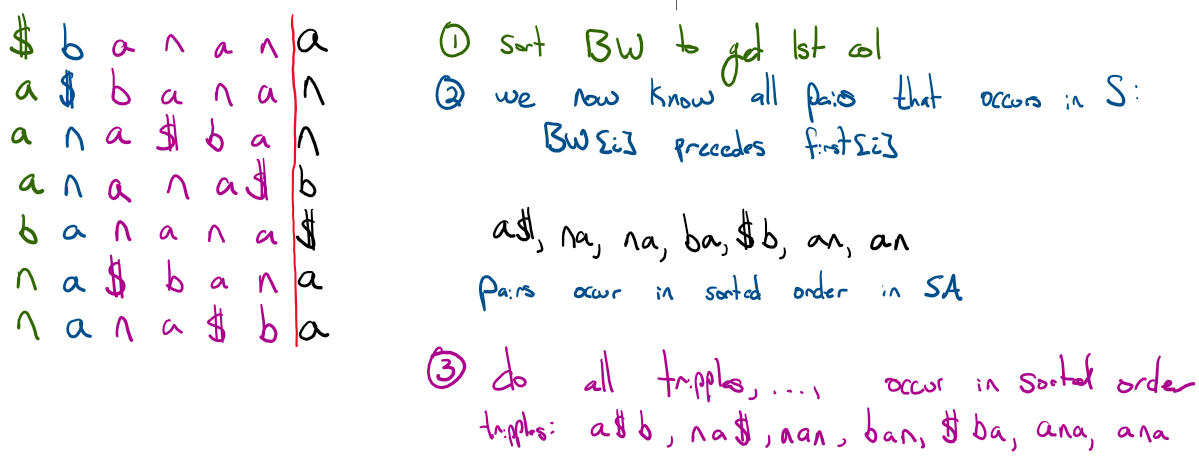
\includegraphics[width=\linewidth]{BWT.png}
\end{figure}

\subsection{FM-Index}
Ferrachina and Manzini.
Consists of 3 parts. 
1) Burrows-Wheeler Transform (BMT), 
2) Count Array $C$, $C[x] =$ number of letters in S lexicographically less than x
3) occ(x, i) = number of x's in BW[1 \dots i].
This uses O(n) space

Lemma: if range(Q, S) = [st, ed]. Then range(xQ, S) = [a, b], 
where $a = C[x] + occ(x, st-1)$, and $b = C[x] + occ(x, ed)$.
This leads to backwards search alg to find occurrences of Q in S.

\begin{algorithm}[H]
    \begin{algorithmic}[1]
    %\algsetup{linenosize=\tiny}
    \tiny
    \Function{FM-Backwards-Search}{$Q, S$}
        \State $st=1$, $ed=n$, $i=|Q|=m$
        \While{$st \leq ed$ and $i \geq 1$}
            \State $x = Q[i]$, $i = i-1$
            \State $st = C[x] + occ(x, st-1) + 1$
            \State $ed = C[x] + occ(x, st-1)$
        \EndWhile
        \If{$st \leq ed$}
            \State return [st, ed]
        \Else
            \State return not found
        \EndIf
    \EndFunction
    \end{algorithmic}
\end{algorithm}

\section{MSA}
Goal is to optimally align multiple sequences at once.
Sum of Pairs scoring $SP(a_1, \dots, a_k) = \sum{1 \leq i < j \leq k} \delta(a_i, a_j)$.
Standard DP uses $O(n^k)$ space, $O(n^k * 2^k *k^2)$ time.
Standard DP can be reformulated into
$$V(i_1, \dots, i_k) = \max_{b_1, \dots, b_k \in \{(0,1)\}^k \setminus (0, \dots, 0)} V(i_1 - b_1, \dots, i_k - b_k) + SP(S_1[i_1 \cdot b_1], \dots S_k[i_k \cdot b_k])$$

Center Star Algorithm, minimize edit distance.
Two approximation algorithm. 
Runs in $O(k^2 n^2)$ time.
\begin{algorithm}[H]
    \begin{algorithmic}[1]
    %\algsetup{linenosize=\tiny}
    \tiny
    \Function{Center-Star}{$S_1, \dots, S_k$}
        \State K = kxk matrix, $K[i,j] = $edit distance between $S_i, S_j$
        \State Compute distance to other strings $D_i = \sum_{j=1}^k K[i,j]$
        \State take center string $S_c$, where $c = argmin_{i} D_i$
        \State Compute alignments with $S_c$
        \State Merge alignments together (need to add spaces)
    \EndFunction
    \end{algorithmic}
\end{algorithm}

\begin{figure}[h] 
    \centering
    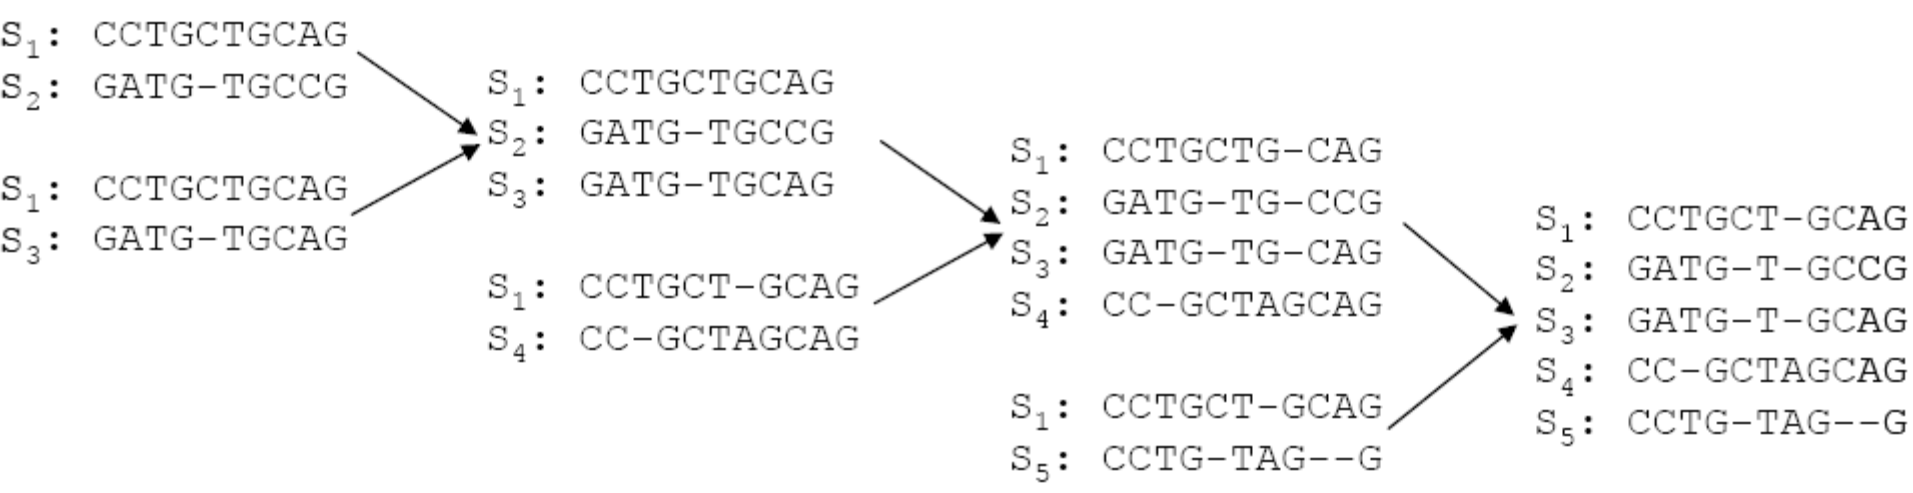
\includegraphics[width= \linewidth]{center_star.png}
\end{figure}


\section{Phylogeny Reconstruction}
Small parsimony problem - given set of S sequences and topology T, find labeling for T that minimizes(?) parsimony.
Solved by Fitch’s algorihtm.
Large parsimony problem - find best topology that minimizes parsimony (NP-HARD).
Two Approximation algorithm. Create complete graph, with edge weight = HammingDist(u, v). Pick T = min spanning tree.


\begin{algorithm}[H]
    \begin{algorithmic}[1]
    %\algsetup{linenosize=\tiny}
    \tiny
    \Function{Fitch's Algorithm}{$T$ - leaf labeled tree, where leaf $v$ is labeled by single char $v_c$}
        \State for every leaf $S_v = \{v_c\}$
        \State for every internal node $v$ with children $u, w$. 
        \State $s_v = \begin{cases}
            S_u \cap S_w & \text{if } S_u \cap S_w \neq \emptyset \\
            S_u \cup S_w & \text{otherwise}
        \end{cases}$
        \For{every node $v$ in pre-order (top down)}
            \State let $u$ be its parent, if $u_c \in S_v$, $v_c = u_c$
            \State otherwise, set $v_c=$ any char in $S_v$
        \EndFor
    \EndFunction
    \end{algorithmic}
\end{algorithm}

\begin{figure}[h] 
    \centering
    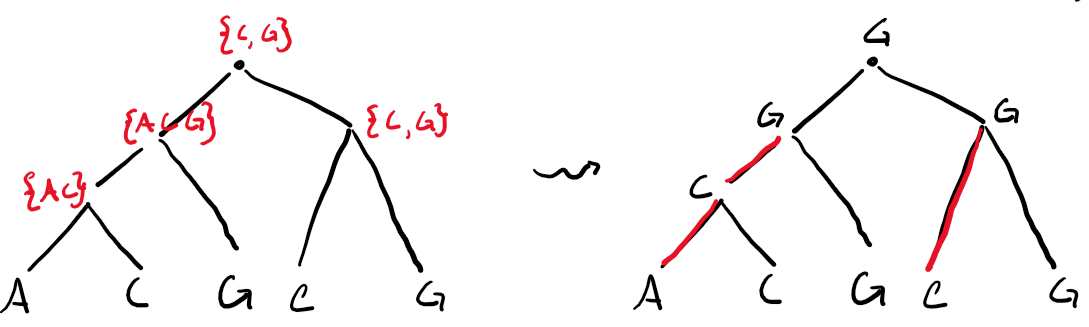
\includegraphics[width=0.7\linewidth]{fitch.png}
\end{figure}

\end{document}